% !!!IMPORTANT NOTE: Please read carefully all information including those preceded by % sign
%Before you compile the tex file please download the class file AIMS.cls from the following URL link to the
%local folder where your tex file resides. http://aimsciences.org/journals/tex-sample/AIMS.cls.
\documentclass{aims}
\usepackage{amsmath}
  \usepackage{paralist}
  \usepackage{graphics} %% add this and next lines if pictures should be in esp format
  \usepackage{epsfig} %For pictures: screened artwork should be set up with an 85 or 100 line screen
\usepackage{graphicx}  \usepackage{epstopdf}%This is to transfer .eps figure to .pdf figure; please compile your paper using PDFLeTex or PDFTeXify.
 \usepackage[colorlinks=true]{hyperref}
   % Warning: when you first run your tex file, some errors might occur,
   % please just press enter key to end the compilation process, then it will be fine if you run your tex file again.
   % Note that it is highly recommended by AIMS to use this package.
   \hypersetup{urlcolor=blue, citecolor=red}
%\usepackage{hyperref}

  \textheight=8.2 true in
   \textwidth=5.0 true in
    \topmargin 30pt
     \setcounter{page}{1}

% The next 5 line will be entered by an editorial staff.
\def\currentvolume{X}
 \def\currentissue{X}
  \def\currentyear{200X}
   \def\currentmonth{XX}
    \def\ppages{X--XX}
     \def\DOI{10.3934/xx.xxxxxxx}

 % Please minimize the usage of "newtheorem", "newcommand", and use
 % equation numbers only situation when they provide essential convenience
 % Try to avoid defining your own macros

\newtheorem{theorem}{Theorem}[section]
\newtheorem{corollary}{Corollary}
\newtheorem*{main}{Main Theorem}
\newtheorem{lemma}[theorem]{Lemma}
\newtheorem{proposition}{Proposition}
\newtheorem{conjecture}{Conjecture}
\newtheorem*{problem}{Problem}
\theoremstyle{definition}
\newtheorem{definition}[theorem]{Definition}
\newtheorem{remark}{Remark}
\newtheorem*{notation}{Notation}
\newcommand{\ep}{\varepsilon}
\newcommand{\eps}[1]{{#1}_{\varepsilon}}

% This is for Pandoc Markdown -> LaTeX, but AIMS author guidelines do not allow
% custom LATeX macros except for equations!
%\providecommand{\tightlist}{%
%  \setlength{\itemsep}{0pt}\setlength{\parskip}{0pt}}
%
%  


%% Place the running title of the paper with 40 letters or less in []
 %% and the full title of the paper in { }.
\title[Teaching Data Science in
Biology] %Use the shortened version of the full title
      {Teaching Data Science to Students in Biology using R, RStudio and
Learnr: Analysis of Three Years Data}

% Place all authors' names in [ ] shown as running head, Leave { } empty
% Please use `and' to connect the last two names if applicable
% Use FirstNameInitial.  MiddleNameInitial. LastName, or only last names of authors if there are too many authors
\author[Guyliann Engels, Philippe Grosjean and Frédérique Artus]{}

% It is required to enter 2020 MSC.
\subjclass{Primary: XXXXX; Secondary: YYYYY.}
% Please provide minimum  5 keywords.
 \keywords{Data Science Teaching, Flipped Classroom, R, RStudio, git.}

% Email address of each of all authors is required.
% You may list email addresses of all other authors, separately.
 \email{Guyliann.Engels@umons.ac.be}
 \email{Philippe.Grosjean@umons.ac.be}
 \email{Frederique.Artus@umons.ac.be}

% Put your short thanks below. For long thanks/acknowledgements,
%please go to the last acknowledgments section.
%\thanks{We would like to acknowledge...}

% Add corresponding author at the footnote of the first page if it is necessary.
% Please add <dollar>^*<dollar> adjacent to the corresponding author's name on the first page.
% The example shown in this template is if the first author is the corresponding author.
\thanks{\textsuperscript{*} Corresponding author: Guyliann Engels}

\begin{document}
\maketitle

% Enter the first author's name and address:
\centerline{\scshape Guyliann Engels\textsuperscript{*}, Philippe Grosjean}
\medskip
{\footnotesize
% please put the address of the first author
 \centerline{Numerical Ecology Department, Complexys and InforTech Institutes, University of Mons}
   %\centerline{Other lines}
   \centerline{Avenue du Champ de Mars, 8, 7000 Mons, Belgium}
} % Do not forget to end the {\footnotesize by the sign }

\medskip

\centerline{\scshape Frederique Artus}

\medskip
{\footnotesize
 % please put the address of the second  and third author
 \centerline{ Pedagogical Support and Quality Assurance Department, University of Mons}
  % \centerline{Other lines}
   \centerline{Place du Parc, 20, 700 Mons, Belgium}
}

\bigskip

% The name of the associate editor will be entered by an editorial staff
% "Communicated by the associate editor name" is not needed for special issue.
% \centerline{(Communicated by the associate editor name)}


%The abstract of your paper
\begin{abstract}
  We examine the impact of implementing active pedagogical methodologies
  in three successive data science courses for a curriculum in biology
  at the University of Mons, Belgium. Blended learning and flipped
  classroom approaches were adopted, with an emphasis on project-based
  biological data analysis. Four successive types of exercises of
  increasing difficulties are proposed to the students. Tutorials
  written with the R package learnr are identified as a critical step to
  transition between theory and application of the concepts. Cognitive
  workload to complete the learnr tutorials is measured for the three
  courses and is only lower for the last course, suggesting students
  need a long time to get used to their software environment (R, RStudio
  and git). A comparison between final summative assessment and grading
  of applied biological data analysis (projects) shows a low
  correlation. This suggests that the final exam does not assess
  practical skills very well. The final exam was dropped at the benefit
  of an ongoing assessment. Data relative to students' activity,
  collected primarily for the ongoing assessment, are also used to
  establish profiles of the students according to their learning
  strategies. Several suboptimal strategies are observed and discussed.
  Finally, the timing of students contributions, and the intensity of
  teacher-learner interactions related to these contributions are
  analyzed before, during and after mandatory distance learning due to
  COVID-19 lockdown. A lag phase was visible at the beginning of the
  first lockdown, but the work of the students was not markedly affected
  during the second lockdown period that lasted much longer.
\end{abstract}

\hypertarget{introduction}{%
\section{Introduction}\label{introduction}}

In a context where there is an exponentially growing mass of data
\cite{Marx2013}, a reproducibility crisis in Science \cite{Baker2016},
and a progressive adoption of Open Science practices \cite{Banks2019},
statistic is broadened to a wider discipline called Data Science
\cite{Cleveland2001}. For the Data Science Association, ``the Data
Science means the scientific study of the creation, validation and
transformation of data to create meaning''
(\url{http://www.datascienceassn.org/code-of-conduct.html}). These
changes also led to the emergence of data science programs in
universities and higher schools \cite{Donoho2017, Cetinkaya-Rundel2021}.
One example is the Harvard Data Science initiative
(\url{https://datascience.harvard.edu/about}) launched in 2017. With a
broader approach, also comes a broader audience. Such data science
courses are not limited to computer scientists, mathematicians or
statisticians. Students in humanities, social sciences, and natural
sciences also attend them (for instance, the data science training at
Duke University \cite{Cetinkaya-Rundel2021}). The focus of such courses
is for students to develop the ability to deal with real datasets in all
their complexities, to be able to conduct reproducible analyses, and to
interpret these analyses in the light of knowledge in their field of
expertise.

These data science courses pose several pedagogical challenges because
numerous and unfamiliar concepts must be acquired by a heterogeneous
class population \cite{Guzman2019}. Learning objectives span a large
range of cognitive abilities and, in these courses, the intended
learning outcomes aim to develop high-level cognitive process abilities
such as conceptual, procedural, and even metacognitive knowledge
\cite{Krathwohl2002}. To meet such learning objectives, active learning
methods are useful so that students could better acquire these
high-level cognitive skills \cite{Freeman2014}. Advances in educational
psychology, reviewed by Kirchner \& Hendrick \cite{Kirschner2020}, give
a scientific background to understand why a pedagogical practice works
or not. Many teaching and learning frameworks involving numerical tools
turn to a blended learning scenario including remote activities to be
done before and after in-class work, individual and group
problem-solving, peer instructions and ongoing assessment. The flipped
classroom approach also involves a mix between at home and in class
activities, but learning occurs before the classes that are dedicated to
discussions and problem solving. This allows students to be active in
their learning, which has the benefit of improving student competences
\cite{Freeman2014}. Moreover, this approach enables students to work at
their own pace. Their diverse learning strategies are respected as they
are actors in their learning process \cite{Spadafora2018}. Such
frameworks are open learning centered, and are supported by a varied and
rich pedagogical environment \cite{Burton2011}.

The data transformation part of the process in data science is a
challenge for students with little or no background at all in computing
sciences. Students that do not master one or more computer languages
enter an unfamiliar world and have to deal with many exotic concepts,
techniques and tools. Version control systems like git, and their
Internet hosting counterparts like GitHub, Gitlab or Bitbucket are also
tools that are taught and used in data science courses
\cite{Fiksel2019, Hsing2019}. The use of document formats that
dissociate content from presentation, namely LaTeX, Jupyter Notebook, R
Markdown or Quarto to cite a few, also contribute to the large number of
potentially new tools learners have to discover \cite{Baumer2014}. On
the other hand, a student in computing science already masters one or
more computing languages. He or she is acquainted with version control
systems, with databases and with the way data are manipulated and
represented in a computer. Yet, the same student in computing science
could have difficulties grasping the context of the study related to
foreign disciplines. A student in mathematics or statistics is familiar
with various concepts that underpin the techniques used to analyze the
data. Students in biology, medicine, psychology, social sciences,
economics, \ldots{} have obviously very different \emph{a priori}
knowledge. The gap between knowledge and learning outcomes generates
anxiety (see for instance \cite{Onwuegbuzie2003}). The course must thus
be organized in a way that learners progress by little steps to avoid
exposure to too many intimidating concepts and tools at once, taking
into account their respective \emph{a priori} knowledge and their
initial gaps.

Suitable computer hardware and software environments are required to
apply the concepts learned in data science courses. Different approaches
range from using software accessed from a server \cite{Theobold2021}
(RStudio Cloud (\url{https://rstudio.cloud/} \cite{Rstudio2015}),
Chromebook data science
(\url{http://jhudatascience.org/chromebookdatascience/})) to local
installation on the student's computers. The former requires
infrastructure to run the software on a server, and that software is
only accessible to the students during the course. The latter raises
problems of license for proprietary software but also installation and
configuration issues. An intermediary solution uses preconfigured
virtual machines, or containers (e.g.~Docker)
\cite{Cetinkaya-Rundel2018, Boettiger2015}. Such a solution is the most
flexible one because it can be deployed almost anywhere (in the computer
lab, at home, on a laptop, \ldots). As practical applications are
important to learn data science \cite{Larwin2011}, a correct choice of
software is critical. Exposing students early with the tools they are
most susceptible to use later in their work is desirable. This was
highlighted by Auker and Barthelmess \cite{Auker2020} for instance, for
ecologists and by Alvarenga da Silva and Sampaio Moura
\cite{Alvarenga2020} for physicians.

Recently, data science has also been used to analyze the effect of
various pedagogical practices on the outcome of these courses thanks to
learning analytics \cite{Estrellado2020}. A vast amount of data can be
collected about students' activities, and the analysis of these data
allows comparing the impact of different pedagogical approaches, or to
quantify and document the impact of such changes in the courses
\cite{Romero2020}.

At the University of Mons in Belgium (UMONS), we reworked our
biostatistics courses in the biology curriculum in 2018. A series of
Data Science courses were introduced, both for our undergraduate and
graduate students. The goal of these courses was to form biological data
scientists capable of extracting meaningful information from raw
biological data. They must be able to do so in a reproducible way and
with the correct application of statistical tools and an appropriate
critical mind. The goal was thus vastly broaden, and it did not solely
targets skills in biostatistics any more.

The learning outcomes defined for these Biological Data Science courses
were thus to be able to analyze most recurrent biological data in
practice and to present the results clearly and accurately in a
scientific report. In order to achieve these learning outcomes the
students had to master skills in biostatistics, scientific writing and
they had to become proficient in the use of computer tools like R,
RStudio, git, GitHub and R Markdown. They also had to develop a critical
mind in statistical thinking. All these learning outcomes are described
in the students' study programme at UMONS, see for instance for the
academic year 2020-2021 \cite{ds1bio2021, ds2bio2021, ds3bio2021}. A
preconfigured VirtualBox machine with R, RStudio, R Markdown, git, and a
series of preinstalled R packages is used
(\url{https://www.sciviews.org/software/svbox/}) as a convenient mean to
deploy the same software environment both on the university computers
and on the student's own laptops.

As our courses were reworked, we also decided to use flipped classroom
and progressive adoption of suitable pedagogical practices in that
particular context with a cyclical approach that consists of stating
goals, building pedagogical material with a large emphasis on numerical
tools and collection of students' activities, and finally, analysing the
data collected. This approach let us enhance our teaching activities the
following academic year with improved pedagogical techniques. This
approach is known as educational data mining knowledge discovery cycle
\cite{Romero2020}. Here, we present the main results spanning on three
successive academic years from 2018-2019 to 2020-2021, including two
particular periods where distance learning was forced due to COVID-19
pandemic lockdown. In this paper, we will focus on the following three
questions:

\begin{itemize}
\item
  Transition from theory to practice is critical and tutorials built
  with learnr (\url{https://rstudio.github.io/learnr/}) are capstones in
  our courses. What cognitive workload and perceived workload do these
  tutorials represent for the students?
\item
  How could we use learning analytics to spot suboptimal learning
  strategies and discriminate different student profiles in our
  biological data science courses?
\item
  Did the quick shift from face-to-face to distance learning imposed by
  COVID-19 lockdown periods affected the production of our students and
  did it require increased exchanges with the teaching staff to support
  it?
\end{itemize}

\hypertarget{methods}{%
\section{Methods}\label{methods}}

This study focuses on three successive courses of increasing
difficulties, called here A, B and C and designed as a continuum. These
courses were part of the core curriculum and were thus mandatory for all
students enrolled in the Bachelor, or Master in Biology at UMONS.

\begin{itemize}
\item
  Course A was about data preparation, description and visualization. It
  also introduced inference with most common hypothesis tests in biology
  (\emph{t} test, ANOVA, \ldots). It was taught in the second year of
  the Bachelor. Course A was set up to assume only background knowledge
  acquired by the students during their first year of the same Bachelor
  in Biology at UMONS.
\item
  Course B taught data modeling (linear, generalized linear and
  nonlinear models) and multivariate analyses (PCA, MDS, clustering,
  \ldots) to students enrolled in the third year of the Bachelor in
  Biology at UMONS. Course A is a prerequisite (all students following
  course B have previously passed course A).
\item
  Course C was taught to all Master students in the Biology section
  (first year of the Master). This course focused on machine learning,
  time series analysis and the analysis and visualization of
  georeferenced data. These students had either passed both course A and
  B at UMONS, or they demonstrated similar knowledge. Only a very few
  number of students (only one in 2020-2021 on a total of 26 students)
  came from a different Bachelor and had thus different courses that A
  and B in their cursus.
\end{itemize}

The course material is available online (\url{https://wp.sciviews.org})
and is centralized in a Wordpress site. Students had to login with their
GitHub account and their academic data were collected from the UMONS
Moodle server (\url{https://moodle.umons.ac.be}). The courses were
broken down into modules that amount roughly to 15h of work each. There
were two in-class sessions of 2h and 4h per module (outside lockdown
periods, of course). There was roughly 3h of preparation at home before
each session, and 3h of work to complete one module. The main activities
in the class were analysis of actual data (projects). Students also
asked questions and followed brief lectures (1/4 h) on selected topics
in the class. They had to propose and vote for the topics to be covered
during these short lectures. Finally, we encouraged students to help
each other and to explain what they understood to their colleagues.
Indeed, students' questions were sometimes redirected by the teacher to
other students that had already mastered the topic. Teachers rarely
answered questions directly. When it was possible, they rather proposed
new tracks or ideas to investigate and helped learners to find the
solution by themselves. Students who went through the activities before
the others were also encouraged to help their slower colleagues.

Regarding the timing, one module was taught every second week so that
students had enough time to prepare the material at home before in-class
session, and after it, to finalize their projects for the module. As a
term is made of 14 weeks, we did not teach more than six modules in a
course unit to avoid compacting them too much in time. After reading the
theory, students were exposed to exercises of four increasing levels of
difficulty. They thus had to apply the concepts repeatedly but in
different contexts, which broke monotony and maintained a stimulating
rhythm all along their progression. They had to learn the principles in
the online book (\url{https://wp.sciviews.org}) and self-assessed their
comprehension of the concepts using H5P (\url{https://h5p.org})
exercises (level 1 difficulty). These exercises were simple questions
(TRUE/FALSE, multiple choice,\ldots). Learnr tutorials
(\url{https://rstudio.github.io/learnr/} were used for the level 2
exercises. They were gently introducing the students to the R code
required for the analyses and guided them step by step through their
first data analysis. These tutorials were thus the entry point to the
practice.

Most of the practical work was dedicated to GitHub projects (level 3 and
level 4 difficulties). At this stage, the use of R instructions was not
sufficient to complete the exercises. Students had to also become
acquainted with git, GitHub, R Markdown and RStudio to manage the
projects. They also had to interpret the results they obtained. The
individual projects (level 3) contained guidance on how to perform the
different step of the analyses. The group projects (level 4, groups of
two or four students) did not contain such guidance. At level 3, goals
were clearly specified in the projects. At level 4, students had to
imagine suitable biological and statistical questions that could be
answered by analyzing the data proposed in the project. Working on these
projects represented both the core of in-class activities and the best
expression of their learning progression. By construction, level 1 to
level 4 exercises are built according to increasing cognitive
difficulties following bloom's taxonomy \cite{Krathwohl2002}.

All students' activities in H5P exercises (self-assessing), and in
learnr tutorials (transitioning smoothly from theory to practice) were
recorded in a MongoDB database. The \{learnitdown\} R package
(\url{https://www.sciviews.org/learnitdown/}) provides the code required
to manage user login, user identification and activity tracking for this
interactive material.

Projects containing the data, the analyses and the reports were hosted
in GitHub repositories. These repositories were cloned and edited by the
students in their virtual machines (SciViews Box) with RStudio
(\url{https://www.rstudio.com/products/rstudio/}), either on their
laptops or on the computers in the lab. We encouraged our students to
install the virtual machine for the course on their own computer so that
they were able to work comfortably at home and could also use it for
other activities too. Assignment and creation of the GitHub repositories
for each student, or group of students, was orchestrated by GitHub
Classroom (\url{https://classroom.github.com}). Reports were written in
R Markdown (\url{https://rmarkdown.rstudio.com/}), a file format that
combines the prose with R code to produce analyses results, plots and
tables directly inside the documents. All repositories were ultimately
cloned by the teacher in a centralized area on our servers and data
about commits (git logs) were collected using git version 2.31.1 and R
version 4.0.5 \cite{Rcoreteam2021}. To give an idea of the data recorded
in 2020-2021, we had a little bit more than 3,500 events that were
recorded for each student.

In distance learning, students' support was done via email and Discord
(\url{https://discord.com}). At the end of an academic term, all
recorded messages were collected into text files. These files were
scraped using custom R code to create a table with key information
(basically, who, when, and what) for each message. Surveys were done
periodically in class through Wooclap questionnaires
(\url{https://www.wooclap.com}). Such questionnaires were used to query
perceived workload of the learnr tutorials. Results were manually
exported out of Wooclap by means of Excel files. These data were then
incorporated into a table in our database thanks to an R script.

Data about users, courses, lectures and projects, as well as grading
items (on average, more than 130 grading items were established for each
student in 2020-2021) were pseudonymised: names, emails and all the
personal information were replaced by random identifiers. The different
tables were ultimately exported into CSV files and made public
\cite{Grosjeandataset2020}. Data collection, treatment, and use respect
European GDPR (General Data Protection Regulation) since each student
had to agree explicitly with the way data were collected and used
(including for research purpose) before each course started. They were
able to visualize their data through personalized reports at any time.

The course material was organized in a way that favors autonomy and
self-assessment (direct feedback in the exercises, hints and retry
buttons in case of wrong answers). Table
\ref {tab:tab_ex_levels_summary} summarizes the main characteristics of
the exercises according to the difficulty level.

\begin{table}

\caption{\label{tab:tab_ex_levels_summary}\label{tab:tab_ex_levels} Four levels of increasing difficulties in the exercises.}
\centering
\begin{tabular}[t]{l|l|l}
\hline
Level & Description & Type\\
\hline
L1 & Interactive exercise in the course, direct feedback & h5p\\
\hline
L2 & Tutorial with guided exercises, feedback and hints & learnr\\
\hline
L3 & Individual and guided data analysis & individual project\\
\hline
L4 & Free data analysis and reporting (by 2 or 4 students) & group project\\
\hline
\end{tabular}
\end{table}

R and tidyverse \cite{Wickham2019} packages
(\url{https://www.tidyverse.org}) were used to prepare the data and the
analyses. All three years of pseudonymised data are available in Zenodo
\cite{Grosjeandataset2020, Grosjeandataset2019, Grosjeandataset2018}. A
GitHub repository with the code used to create the figures and table in
this paper is available at
\url{https://github.com/BioDataScience-Course/teaching_data_science_in_biology}.

\hypertarget{measured-and-perceived-cognitive-workload-in-learnr-tutorials}{%
\subsection{Measured and perceived cognitive workload in learnr
tutorials}\label{measured-and-perceived-cognitive-workload-in-learnr-tutorials}}

The average number of trials that were required for each student to find
the right answer in learnr tutorial exercises was used as a proxy of
measured workload. In comparison, the perceived cognitive workload was
established with a NASA LTX questionnaire. This questionnaire is
composed of six questions on a Likert scale \cite{Hart1988}. The
questions concern mental load, physical load, time pressure, expected
success, effort required, and frustration experienced during the
accomplishment of the task. The average value for the six questions
constitutes a Raw Task Load indeX (RTLX) \cite{Byers1989} that we used
to quantify how students felt when using these learnr tutorials. An
analysis of variance and a Tukey's post-hoc Honest Significant
Difference (HSD) tests were used for the comparison between courses.

\hypertarget{students-activity-profiles-with-ongoing-assessment}{%
\subsection{Students activity profiles with ongoing
assessment}\label{students-activity-profiles-with-ongoing-assessment}}

Data from the L1-L4 exercises and the student's support (email and
Discord) were used to characterize the student's activity profiles. A
non-supervised classification technique called Self-Organizing Map (SOM)
\cite{Kohonen1995} was used to characterize various learning profiles.
The \{kohonen\} R package was used to compute the model
\cite{Wehrens2018}.

\hypertarget{transition-between-face-to-face-to-distance-learning-imposed-by-covid-19-lockdown}{%
\subsection{Transition between face-to-face to distance learning imposed
by COVID-19
lockdown}\label{transition-between-face-to-face-to-distance-learning-imposed-by-covid-19-lockdown}}

The transition between face-to-face to distance learning was studied
through the contribution of each student in projects with the commits
(git logs) and by these contributions divided by the questions they
asked by email and on Discord. Only descriptive analysis of these data
was done, but interesting patterns were observed.

\hypertarget{results}{%
\section{Results}\label{results}}

This study was performed on data related to the three successive courses
that comprise 26 modules in total in 2020-2021. Table
\ref {tab:tab_course} summarizes the number of H5P, learnr, individual
and group GitHub projects that students had to complete. Group projects
usually spanned over several modules. It should be noted that for course
C, we also introduced a challenge in machine learning that replaced one
group GitHub project. This challenge is omitted from the present
analysis, being a unique activity that is difficult to compare to the
rest. However, this explains why there was only one group project in
course C.

\begin{table}

\caption{\label{tab:tab_course_summary}\label{tab:tab_course} Number of students, modules, and exercises for each course. For the learnr tutorials, the first number is the amount of tutorial documents and the second number in brackets is the total number of questions in these tutorials (year 2020-2021).}
\centering
\begin{tabular}[t]{l|r|r|r|l|r|r}
\hline
Course & Students & Modules & H5P & Learnr & Indiv. projects & Group projects\\
\hline
A & 59 & 12 & 59 & 24 (211) & 10 & 4\\
\hline
B & 45 & 8 & 29 & 11 (108) & 12 & 2\\
\hline
C & 26 & 6 & 19 & 7 (37) & 7 & 1\\
\hline
\end{tabular}
\end{table}

Retrospective data from 2018-2019 (only course A)
\cite{Grosjeandataset2018} and 2019-2020 (courses A and B)
\cite{Grosjeandataset2019} were also used when it was pertinent. For
instance, final exams were only used during these two years. It should
be kept in mind that the pedagogical material was written and improved
progressively during the three academic years. The H5P exercises and the
auto-checking of learnr answers were not available before 2020-2021. We
do not use data corresponding to our former courses in biostatistics
that were given in a more traditional way because we consider the
comparison would not be unbiased: the content of these courses was quite
different. However, experience gathered with these former courses for 15
years was critical in the redesign of the new ones.

\hypertarget{measured-and-perceived-cognitive-workload-in-learnr-tutorials-1}{%
\subsection{Measured and perceived cognitive workload in learnr
tutorials}\label{measured-and-perceived-cognitive-workload-in-learnr-tutorials-1}}

In our courses, learnr tutorials help students to transition from the
theory (online book chapters) to the practice (projects). These
tutorials are online interactive documents that recall main concepts,
and take the students by the hand to perform their first data analysis
step by step. At each step, they have at least one exercise or one quiz.
The exercise consists in writing R code, or filling missing parts in R
code to progress in the analysis.

Our goal with these tutorials was to optimally prepare the students for
the practice of data science. The usefulness of these tutorials was
qualitatively determined by observing the behavior of the students when
they started their practical work. On the other hand, the number or
retries necessary to complete an exercise on average, the number of
exercises correctly answered, or the time needed to complete one
tutorial are quantitative measurements and could be analyzed in order to
optimize these tutorials.

A few tutorials were elaborated during the academic year 2018-2019, and
positive feedback on their utility (both by direct observation of the
students and thanks to their remarks) led us to systematize them into
what we now call level 2 activities (see Table \ref {tab:tab_course}) in
the form of learnr documents in 2019-2020. The tutorials were further
refined in 2020-2021: we added contextual hints with the \{gradethis\} R
package (\url{https://pkgs.rstudio.com/gradethis/}). In their latest
version, when students submit their answer to the exercises, the R code
is parsed, analyzed and the result is compared with the solution. In
case of differences, heuristics are used to provide contextual hints.
Students can then refine their solution and resubmit it. This appears
very efficient in self-learning and self-assessing their competences
before switching to the practice with confidence.

\begin{figure}
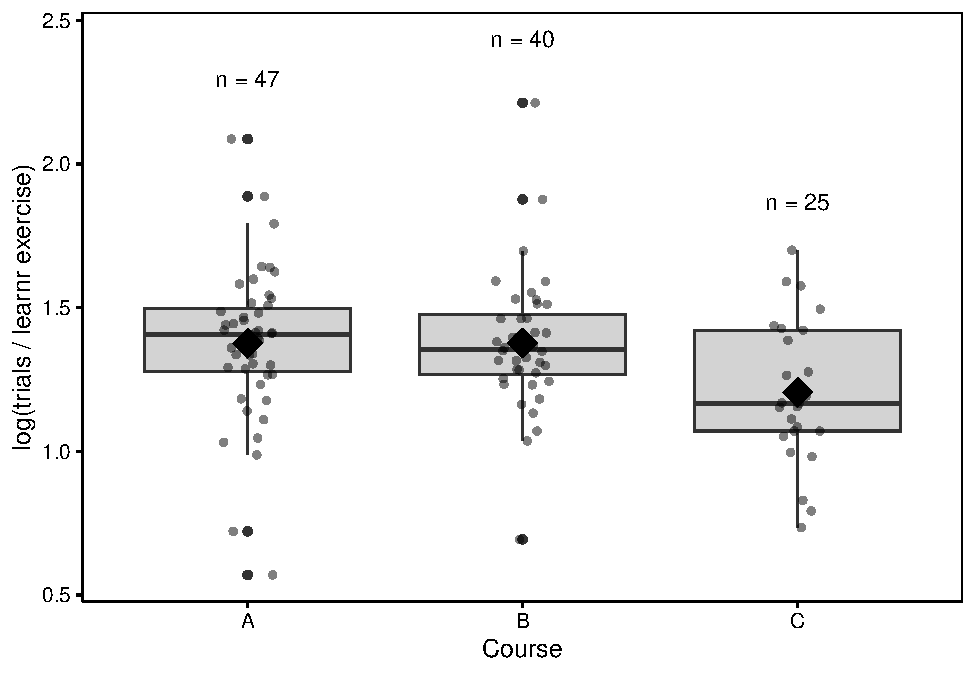
\includegraphics[width=1\linewidth]{teaching_data_science_files/figure-latex/fig_learn_trials-1} \caption{\label{fig:fig_learn_trials} Logarithm of the average number of retries that were required for each student to find the right answer in learnr tutorials exercises (year 2020-2021). This measure is used as a proxy to quantify the cognitive workload (with caution as explained in the text). The black dot is the average for the whole class and n is the number of observations.}\label{fig:fig_learn_trials}
\end{figure}

A fully objective quantitative measurement of the cognitive workload is
near to impossible to obtain in these asynchronous activities done at
home. It was thus estimated by using a proxy: the logarithm of the
average number of trials that were required for each student to find the
right answer in learnr tutorial exercises (Fig.
\ref {fig:fig_learn_trials}). Caution is required here as a large number
of trials could also be the result of students that are just guessing.
However, answers being pieces of R code, pure guessing most probably
leads to nothing useful. A certain level of understanding of both the R
syntax and the question are required to obtain correct answers. Only
data from students that correctly answered most of the exercises
(\textgreater{} 90\%) were used here, as it also rules out the students
that appear to have insufficient knowledge to master the concepts in the
tutorials and are probably just guessing. For course A, 12 out of 59
students did not pass this filter, 5 out of 45 for course B and 1 out of
26 for course C. This variable varies significantly between the three
courses (ANOVA, F(2, 109) = 4.49, p-value = 0.013). The homogeneity of
variances (Bartlett Test, K2 = 0.30, df = 2, p-value = 0.86) and the
Normal distribution of the residuals using a quantile-quantile plot were
verified. The students in course C need significantly fewer trials to
find the right answer than students in courses A at \(\alpha\) level of
5\% (Tukey HSD, t = -2.74, p-value = 0.019) and B (Tukey HSD, t = -2.68,
p-value = 0.023).

The perceived cognitive load required to perform these exercises was
also determined on the same students and for the same exercises. The Raw
Task Load indeX (RTLX) measured the emotional state of the students
after having completed a tutorial. This has, as far as we know, not been
done yet. We used a NASA LTX questionnaire to assess it across all three
courses. Participation to the survey was high: 48/59 (81\%), 35/45
(78\%) and 18/26 (69\%) for courses A, B, and C respectively.

\begin{figure}
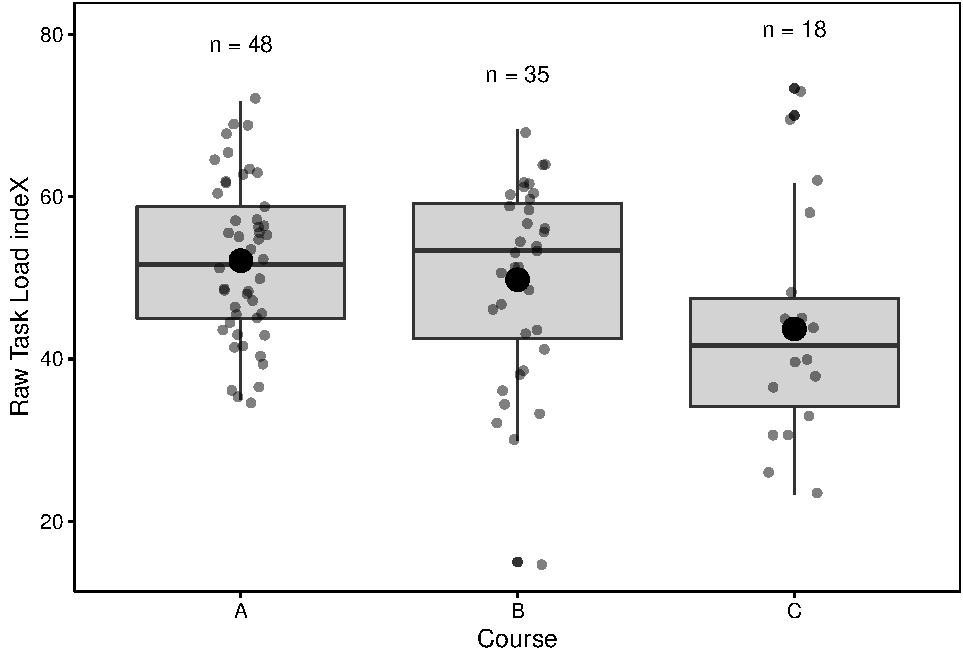
\includegraphics[width=1\linewidth]{teaching_data_science_files/figure-latex/fig_rtlx-1} \caption{\label{fig:fig_rtlx} Perceived workload for the learnr tutorials in the three courses (year 2020-2021). The big black dot is the mean RTLX value. The number above each box is the number of respondants.}\label{fig:fig_rtlx}
\end{figure}

The difficulty of the course, and thus, of the exercises in the
tutorials increased from one course to the other. However, we do not
observe any increase, neither in the number of retries, nor in the RTLX
(Fig. \ref {fig:fig_rtlx}). On the contrary, these appear significantly
lower for course C than for course A at the \(\alpha\) level of 5\%
(ANOVA, F(2, 98) = 3.59, p-value = 0.031; Tukey HSD, t = -2.68, p-value
= 0.023). The homogeneity of variances (Bartlett Test, K2 = 4.17, df =
2, p-value = 0.12) and the distribution of the residuals using a
quantile-quantile plot were verified and indicate that they do not
depart significantly from a Normal distribution. The cognitive load
perceived by the students diminished at the same pace as their ability
to find the right answer in fewer trials. This may be a consequence of a
more fluent R coding ability and a better mastering of the software
environment.

\hypertarget{students-activity-profiles-with-ongoing-assessment-1}{%
\subsection{Students activity profiles with ongoing
assessment}\label{students-activity-profiles-with-ongoing-assessment-1}}

The flipped classroom approach and the proactive attitude we expected
from our learners (they had to formulate questions correctly whenever
they face a problem) led to different and contrasted learning
strategies. Not all students asked questions. Some of them tried to find
solutions on their own. Some others preferred to ask their questions
privately, while others had no problems exposing their difficulties on a
public forum (the Discord channel dedicated to the course). The way and
the timing learners progressed in the exercises also largely varied. The
schedule was not tight and only suggested a rate of progression. No
student was penalized if the exercises were done later, as long as they
were completed before the deadline. As expected, a part of our students
preferred to stick to the proposed schedule, while others procrastinated
and differed the completion of their exercises. Some strategies are
probably more efficient than others. We analyzed records of the
students' activities to distinguish the different learning profiles and
we compared them with the grade they obtained at the end of the course.

In 2020-2021, to support the ongoing assessment without a final exam,
the activity of each student in level 1 (H5P) and 2 (learnr) exercises
were exhaustively recorded in a database. For the GitHub projects
(levels 3 and 4 exercises), the GitHub repositories and the git log data
were analyzed. During lockdown periods, exchange with students and
answers to their questions were exclusively done by email, text or voice
messages on Discord on private or public channels. Students were allowed
to freely choose their favorite tool to interact with the teachers and
between each other. All these exchanges were recorded too.

The degree of completion of all the exercises was used to establish the
final grade for the course, with a much higher weight on individuals and
especially, on group projects. The weight was adjusted from course to
course according to the importance of the different projects, mainly. To
give an idea, for course A second term, level 1 H5P exercises accounted
for 5\%, 10\% for level 2 learnr tutorials, 35\% for level 3 individual
projects and 50\% for level 4 group works. On average, each student
received more than 130 assessment items that accounted for their final
grade. Two third of these assessments were established manually, using
evaluation grids based on their work in the various projects. The
remaining third is made of scores automatically calculated from the
online exercises.

For the three courses, we recorded more than 450,000 events, which makes
on average almost 3,500 events for each student. These data contain
information that we used to characterize the behavior and learning
patterns that the students exhibit. They are summarized into sixteen
metrics.

For H5P exercises:

\begin{itemize}
\item
  trials/H5P ex.: the average number of trials for each H5P exercise
  until the right answer is found (students can retry as much as they
  wish and they have immediate feedback whether their answer is correct
  or not),
\item
  correct H5P ex.: the fraction of H5P exercises that were correctly
  answered.
\end{itemize}

For learnr tutorial exercises:

\begin{itemize}
\item
  trials/learnr ex.: the average number of trials for each learnr
  exercise until the right answer is found (here also, students can
  retry as much as they want), excluding quizzes,
\item
  hints/learnr ex.: in learnr exercises, students can display hints to
  help them to solve the problems (but they lose 10\% of the score for
  the exercise for each hint they reveal). This is the average number of
  hints per exercise that were displayed for each student,
\item
  correct learnr ex.: the fraction of learnr exercises that were
  completed with a correct answer,
\item
  time/learnr ex.: the average time required to finish one learnr
  exercise involving R code writing, thus excluding quizzes.
\end{itemize}

For individual and group projects:

\begin{itemize}
\item
  commits/ind. projects: the average number of commits done by a student
  in one individual project,
\item
  contributions/ind. projects: the number of lines changed -added or
  subtracted- in the R Markdown reports by one student in one individual
  project (this includes embedded R code for the processing, analysis
  and plotting of data),
\item
  commits/group projects: same as above, but for group projects,
\item
  contributions/group projects: same as above, but for group projects,
\item
  percentage of contributions to group projects: the fraction of work
  the student did, relative to all the work done in group projects.
\end{itemize}

For support:

\begin{itemize}
\item
  questions/module: the number of questions students asked, divided by
  the number of modules in the course,
\item
  percent of public questions: the fraction of questions that the
  student posted in a public channel (the Discord channel dedicated to
  the course that all the other students of the class can read),
\item
  contributions/question: a metric that catches the relative
  ``productivity'' of the student related to the number of questions
  they ask.
\end{itemize}

Finally, global measurements:

\begin{itemize}
\item
  work done: the fraction of all exercises that the student completed,
\item
  work done in time: the fraction of exercises done in the right time,
  that is, within the proposed calendar.
\end{itemize}

In our courses, we have a few students in mobility that come from
various origins. The \emph{a priori} knowledge is important in
education. So, to avoid biases due to the past curriculum of the
students, we restrict this analysis to the subpopulation that comes from
the first year of Bachelor in Biology at UMONS only. A Kohonen's
self-organizing map is used to create student profiles according to
their activities (Fig. \ref {fig:fig_som}). A three by three hexagonal
map was chosen, and students are thus classified into nine different
groups.

\begin{figure}
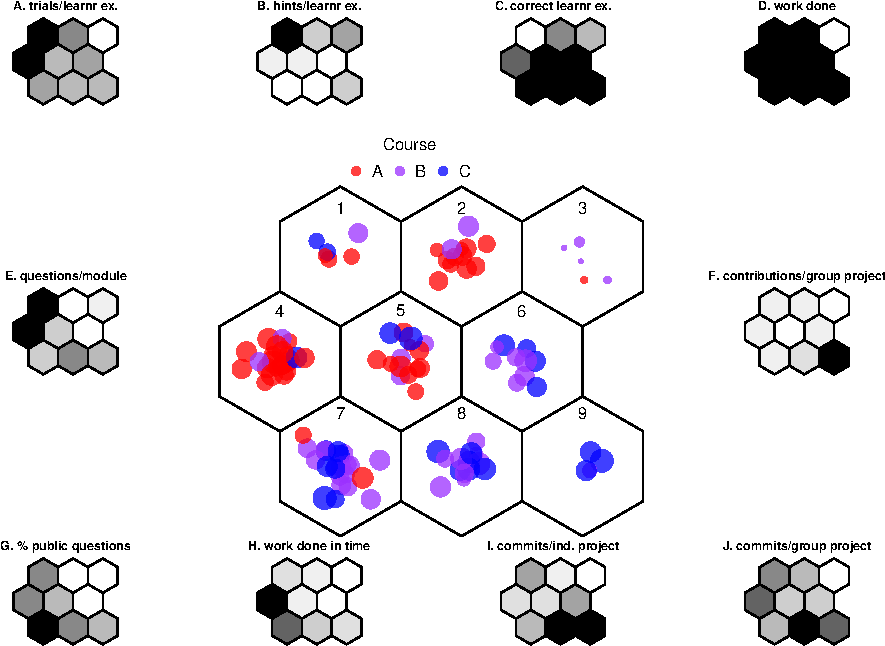
\includegraphics[width=1\linewidth]{teaching_data_science_files/figure-latex/fig_som-1} \caption{\label{fig:fig_som} Self-organizing map of the student activities across the three courses (year 2020-2021). See the text for the explanations.}\label{fig:fig_som}
\end{figure}

In Fig. \ref {fig:fig_som}, the small peripheral plots in gray scale
show how selected metrics distribute in the nine cells, from lowest
value in white to highest value in black. They help to decipher the way
students behave according to their profile. Metrics that are not
represented in the Figure exhibit similar patterns to others (for
instance H5P metrics have a similar pattern to learnr metrics). A table
of the importance of each variable on each cell is presented in the
Appendix. Dots in the central plot are the various students, with color
representing the course and the diameter of the dots indicating the
grade the students obtained at the end of the course. The following
paragraphs detail information in that figure. The numbers between
parentheses are the cell numbers in the central plot, and the uppercase
letters in parentheses refer to the peripheral subplots.

Each cell (1-9) represents a learning strategy used by the students. The
effectiveness of the learning strategy can be determined by the score
obtained. An optimal learning strategy leads to the student achieving a
very high grade. A poor learning strategy leads to the student's failure
(3). Between the two extreme strategies there are several strategies
that are considered suboptimal.

Although most students completed all, or almost all exercises (D), cell
(3) collects the few students that did only a tiny part of these
exercises. These students obtained very low grades, of course. They
belong to courses A and B. On the other hand, heavy workers are at the
bottom (I \& J), and good performers in learnr tutorials (C) are in
cells (5-9).

\begin{itemize}
\item
  Cells (2 and 6) collect students that seldom asked questions (E), and
  that rarely appeared on the public channel (G). Minor differences
  separate them. For instance, learners in cell (2) sometimes used hints
  (B), while those in cell (6) never did so, also because they found the
  correct answer to the exercises more often by themselves (C). Asking
  questions is at the core of our pedagogical approach. So, these
  students did not play the game. However, they were possibly successful
  anyway. Some of them probably exchanged with other students through
  different channels that we did not monitor. Cell (2) -more difficulty
  with learnr tutorials- mainly contains students belonging to course A,
  while cell (6) contains students of courses B and C. There is a clear
  evolution in their behavior from one course to the other in terms of
  ease at realizing the exercises, even if they remain silent at the
  teacher-learner interaction level.
\item
  Among the students that had a hard time to figure out the answers to
  auto-evaluation exercises, cell (1) reassemble people that most
  heavily relied on hints (B), and were among those who had to retry the
  exercises more often before they were figuring out the correct answer
  (A), a characteristic they share with cell (4). These students also
  asked a lot of questions (E), both on the public and private channels
  (G, mid gray indicating a balance between public and private
  messages). The main difference between those two groups is that
  students in cell (4) tried harder to find the answer without looking
  at the hints, while in cell (1) they gave up more rapidly. Also these
  students respected the proposed schedule much more closely than all
  others (H). We have students coming from all courses there, but a
  majority of course A.
\item
  Cells 1-4 plus 6 contain students that exhibit suboptimal behaviors in
  one or the other way. The remaining cells (5, 7-9) correspond to
  learner profiles that perform better from this point of view. Cell (5)
  is primarily represented by students from course A, but secondly, also
  from course B and C. These are average actors in all metrics, except
  they are fluent with level 1 (H5P, not shown) and level 2 (C)
  exercises.
\item
  Moving from cell (5) to (7), (8) and (9), we encounter increasingly
  good performers. The number of students from course A becomes
  progressively lower, while course B, and especially C dominate in
  these groups. In cell (7), they intensively used the public channel
  (G) and also respected the schedule quite well (H) as main differences
  from those from cell (5). Students in cells (8) and (9) were not so
  often in time, but this is because they were heavier workers in the
  projects, both in the individual (I) and in the group (J) activities.
  This needed obviously more time. In cell (9) we also find the students
  that contributed the most to the reports in terms of lines added or
  deleted (F).
\end{itemize}

To summarize, at the top of the SOM map, cells (1-4, plus 6) contain
students with suboptimal behaviors, cell (5) are average students, and
cells (7-9) at the bottom exhibit profiles corresponding to best
performers. The pattern is also visible between courses A (mainly
distributed at the top or center of the map) to B and C (more
represented at the bottom). This probably suggests that students needed
time to get used to the course, its pedagogical approach, and/or the
software environment they had to use. Since only a small fraction of the
participating students failed, excluding the defeating ones in cell (4),
the intercourse pattern can hardly be explained by a filter that
eliminated the low performers from one course to the other.

\hypertarget{transition-between-face-to-face-to-distance-learning-imposed-by-covid-19-lockdown-1}{%
\subsection{Transition between face-to-face to distance learning imposed
by COVID-19
lockdown}\label{transition-between-face-to-face-to-distance-learning-imposed-by-covid-19-lockdown-1}}

Due to COVID-19 lockdown periods, distance learning had to be adopted
abruptly. We analyze the activity collected during academic years
2019-2020 and 2020-2021 to evaluate the impact of these transitions on
the progression of the students. In Fig. \ref{fig:fig_support_by_time},
the academic term is divided into seven work periods of approximately
two weeks each (remind that it was the suggested rate of the courses:
one module every second week). The classes of the second term started at
period~Y1P09, since period~Y1P08 is reserved for the first term exams
session. The courses of the first term of 2020-2021 begun at Y2P01.
First lockdown started at period~Y1P11 for one month and a half. Second
lockdown started at Y2P03 and lasted to the end of the second term
(Y2P15). During the first lockdown, we quickly opened the dedicated
Discord channels that were available without any latency.

\begin{figure}
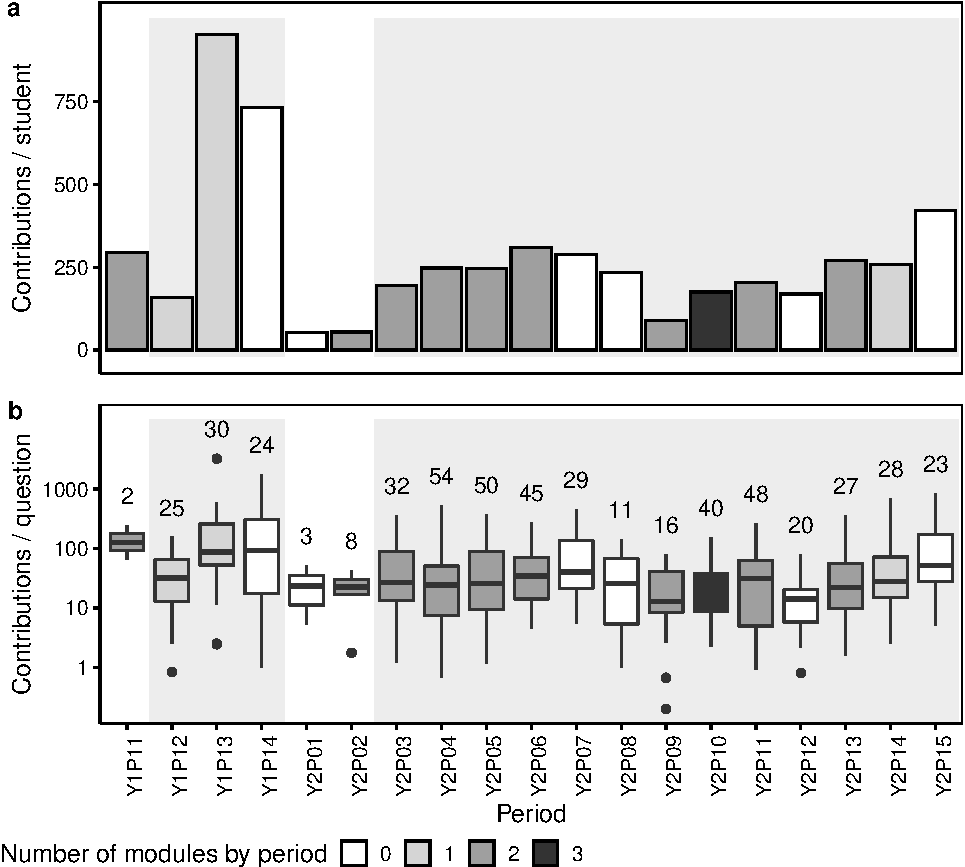
\includegraphics[width=1\linewidth]{teaching_data_science_files/figure-latex/fig_support_by_time-1} \caption{\label{fig:fig_support_by_time} a. Average students' contributions to the projects by periods of two weeks of course. b. Contributions by question asked (log scale) for each student as a measurement of the intensity of teacher-learner interactions relative to the progression. Light gray background indicates periods where distance teaching was mandatory due to COVID-19 lockdown. The number of students that interacted during each period is indicated on top of the boxlots (Y1 is 2019-2020, Y2 is 2020-2021).}\label{fig:fig_support_by_time}
\end{figure}

Contributions per student (Fig. \ref {fig:fig_support_by_time}a) was
relatively constant during the second year, starting essentially at
Y2P03, when the second lockdown was established. The highest activity is
observable at the end (Y2P15), although there was no module taught
during that period. This is because of the late students that finalized
their reports at the last minute. Y2P01, Y2P02 and Y2P09 exhibit the
lowest activity, and these were the start of the first and second terms.
Y2P01 and Y2P01 were also taught in face-to-face and they correspond to
the start of all three courses.

The learners-teachers interactions, especially during the lockdown, is
here quantified by the number of questions. Figure
\ref {fig:fig_support_by_time}b) shows the amount of contributions
divided by the number of questions as a measure of work that was done on
average by the students for each interaction. A higher value means more
autonomy. A lower value indicates more problems or difficulties that
require learners-teachers interactions to be solved. As this measure
spreads over several orders of magnitude from one student to the other,
a logarithmic scale is used. However, median value -the bar inside the
boxes- varies much less. Global number of questions during each period
is less variable, as is the absolute contributions, leading to a rather
stable ratio. The highest median ratios are observed at the last period
of each term (Y2P07 and Y2P15) although no module was taught at that
time. More contributions are observed relative to the questions at the
end: students essentially finalize their reports.

The first year shows a different pattern. First, the lockdown period was
restricted to the very end of the second term. Only the last module in
both course A and B remained. In Y1P12, when distance learning was first
imposed, we observe a marked decrease in the contributions per student
(Fig. \ref {fig:fig_support_by_time}a). It is heavily compensated, and
even overcompensated, in periods~Y1P13 and Y1P14, which are by far the
busiest periods of all. Period~Y1P15 is not represented because it is
after the deadline to finish all work that year.

Intensity of support during the first year shows a similar pattern as
for the second year: extremely widespread from student to student.
Median value is similar too, if not among the highest during
periods~Y1P11, Y1P13 and Y1P14. The productivity was thus not affected
during that first lockdown, after a short lag time observable in Y1P12.

\hypertarget{discussion}{%
\section{Discussion}\label{discussion}}

Teaching data science to a population of students that are not very used
to advanced computer techniques and tools, and that have only basic
knowledge in mathematics and statistics is a hard task \cite{Sousa2018}.
In order to let them learn progressively, the courses were stretched
over a very long period of time: five successive terms spanning on three
consecutive years (undergraduate and graduate). That way, the different
concepts they had to learn were broken down into subunits (26 modules)
that lasted for two weeks each. We also used flipped classrooms and
blended teaching and learning (following Spadafora \& Zopito's
definition of ``any educational model where online delivery ranges from
50\% to 80\%'' \cite{Spadafora2018}), with an emphasis on proactive
exchanges with the teachers: students had to ask questions to progress.
Overall, these appear to be winning choices because most of our students
were successful, excluding a few defeating ones. Compeau also obtained
good results using the flipped classroom with its course targeting
students in biology \cite{Compeau2019}.

Despite our courses framework, students are more used to a traditional
face-to-face approach made of lectures followed by exercises where
important concepts are repeated at the beginning of the practical
sessions. They tend to have a passive attitude during lectures and they
expect teachers and assistants feeding them with the key concepts. That
attitude does not purposely work here. Proactive behavior and
development of autonomy are required \cite{Freeman2014}. They thus have
to engage themselves in a very different way of learning. The transition
between the theory they read in the book and the projects where they
have to apply these concepts is too sharp without a progression that
facilitates students' engagement, in four stages, which are: (L1)
auto-evaluation exercises directly in the online book, (L2) recall of
the main concepts and guided step by step analysis of a first dataset
with the learnr tutorials, (L3) at least one guided individual project
with another dataset, before (L4) they are presented yet a different
dataset to analyse with limited instructions this time.

\hypertarget{measured-and-perceived-cognitive-workload-in-learnr-tutorials-2}{%
\subsection{Measured and perceived cognitive workload in learnr
tutorials}\label{measured-and-perceived-cognitive-workload-in-learnr-tutorials-2}}

The learnr tutorial was immediately spotted as a key activity in the
learning process during academic year 2018-2019. So, we have focused our
attention on these learnr documents. In 2020-2021, the use of a
heuristic engine \{gradethis\} to provide contextual feedback on the
errors students made in their answers was much appreciated.

The number of trials needed to find the right answer is here considered
as a workable proxy for the cognitive workload. Contextual feedback
allowed the student to correct these answers on their own to find the
expected answer. A high number of trials may definitely indicate that
students had a hard time to find the right answer. They could
misunderstand the concepts, but they could also be trying many solutions
at random in order to find the right solution. This indicator alone is
not sufficient, and we combine it with the perceived cognitive workload.
The measured RTLX index will serve in the future as a reference to gauge
possible optimization of the tutorials, with lower perceived workload
without sacrificing the content. The significant decrease in RTLX value
from course A to C indicates that there is still a margin of
progression. We would like to observe such a decrease sooner, perhaps
already in the second course. Monitoring the perceived and measured
cognitive workload is indeed important ``to maintain reflective and
systematic approaches in both the development and evaluation {[}of
our{]} blended approach'' \cite{Spadafora2018}.

\hypertarget{student-activity-profiles-with-ongoing-assessment}{%
\subsection{Student activity profiles with ongoing
assessment}\label{student-activity-profiles-with-ongoing-assessment}}

Activity tracking in the exercises, primarily set up for the ongoing
assessment, also offers the opportunity to study the way learning
happens (or not). Indeed, learning analytics provides opportunities to
monitor learning events but also to adjust teaching to improve student
outcomes \cite{Martin2016, Romero2020}, even if they are primarily used
to early predict success or failure. In our courses, the failure rate
was already rather low and essentially limited to a few defeating
students that did not work at all. We are more interested to classify
our participating students according to their behaviors. This paves the
way toward a more inclusive pedagogy by spotting different kinds of
suboptimal patterns (for instance, never asking questions, looking at
hints too quickly without really trying to figure out the answer, being
shy to discuss problems on public channels, \ldots). Once these patterns
are evidenced, we can then consider countermeasures. As Martin \& Ndoye
highlight from other studies, ``benefits that the online learning
platform provides with respect to assessment include better monitoring
opportunities for student learning and immediate feedback {[}\ldots{]},
and individual practice opportunities'' \cite{Martin2016}. As an example
for students that rarely post their questions publicly, we will test an
alternate discussion channel where teachers never post but have read
access. In case of an error, the teacher will contact the student
privately to explain to him or her what is wrong. That student would
then have the responsibility to reexplain correctly to its classmates.
This way, its error is never publicly spotted by the teacher. With tools
like the self-organizing map, we should be able to predict suboptimal
student profiles early. We could engage in a discussion with the
concerned students to determine the cause and find a solution as early
as possible. Learning analytics used that way would promote a
differential pedagogical approach, a key for more inclusive teaching
\cite{Siemens2013}.

Group projects are one of the keys to our method. Sometimes, groups do
not work well, and one student has to do most of the work. This is a
clear weakness in this approach, especially if one of the defeating
students in Fig. \ref {fig:fig_som} cell (3) is involved. If we could
identify the profile of the different students relatively early during
the course, we would be able to create better groupings with a blend of
different complimentary profiles to enrich the experience of all
learners. Maybe should we work exclusively with groups of four to
mitigate the impact of one defeating student? The balance of
heterogeneous and complimentary competences are essential in such a
group in order to create mutual emulation and efficacy
\cite{Mucchielli1996}. Working on group composition will thus be one of
our future challenges.

\hypertarget{transition-between-face-to-face-to-distance-learning-imposed-by-covid-19-lockdown-2}{%
\subsection{Transition between face-to-face to distance learning imposed
by COVID-19
lockdown}\label{transition-between-face-to-face-to-distance-learning-imposed-by-covid-19-lockdown-2}}

Forced distance learning, due to COVID-19 lockdown did not appear to be
a barrier in the production of our students in their projects. A pattern
is observed during the first lockdown with a marked decrease in their
contributions, followed by a large, compensatory activity. All this
happened in a time frame of a couple of weeks. That was the time needed
to adapt to the new situation. The most problematic aspect was the
access to a powerful-enough computer for roughly 15 to 20\% of our
students. In a normal situation, these students had access to computers
at university, both in-class and outside of class time. When lockdown
was imposed, those students suffered most by a lack of hardware.
However, to reduce the social numeric fracture, the university quickly
reacted and computers were lent to them. During the second lockdown, a
larger part of our students had acquired their own computer, and
solutions were immediately available for the others. Consequently, no
lag time was observed in their production.

If the contributions/questions remained globally at a similar level in
face-to-face or distance learning, their impact on the teacher's
timetables was very different. In distance learning, students worked at
very different moments. Their questions were thus less concentrated
during the course periods. Also, an alternation between asynchronous
work at home and synchronous work in the computer lab is more beneficial
to interactions between students. The social and human components of
teaching and learning are key factors that tend to vanish in exclusive
distance learning. Contacts through videoconferences only partly
compensate for lack of interactions because in-class presence remains
different than video chats. Blended learning combines the best of the
two practices if pedagogical setups are accurate and well balanced
\cite{Bernard2014}.

\hypertarget{conclusion-and-perspectives}{%
\section{Conclusion and
perspectives}\label{conclusion-and-perspectives}}

Teaching data science comes with challenges. The discipline is quite
young, and we are still seeking for the best pedagogical approach. After
three years of teaching data science to undergraduate and graduate
students in a curriculum in biology with revised pedagogical practices,
we have had our first cohort that passed all three courses. There are
still two optional courses available in the second year of the Master if
they want to push their data science skills further on. However, the
three mandatory courses are designed to be self-supported. Globally,
most students acquired the expected competences during these courses. We
have the feeling that they are more mature and more capable in data
science by effectively acquiring the intended outcomes than with our
previous courses in biostatistics given in a more traditional way. The
impact of the revised approach to teach biological data science on the
way learners manage data and data analysis will be observable during the
following years. We will monitor how these students apply their skills
in their master's thesis, and later, in their career or during their PhD
thesis. Meanwhile, we will continue to improve our courses by further
exploiting the data we accumulate on the activity of our students.
Experience gathered during forced distance learning during COVID-19
lockdown will be used too to improve our courses framework. The radical
changes that were required in that context showed that students can
accommodate to a large extent, but also that the diversification of the
activities is beneficial to guarantee their engagement
\cite{Spadafora2018, Young2002}. Speaking about diversification, in
2020-2021 we successfully tested a kaggle-like challenge
(\url{https://www.kaggle.com/competitions}) in one of the machine
learning modules. Such playful activities would also contribute to the
diversification of pedagogical practices, interest and motivation of the
students \cite{Alonso2019}. We would also be happy to share experience
with other teachers in data science. Altogether, we are on the way to
reshape the post-COVID teaching landscape, and it will probably be quite
different than what we were used to!

% You may incorporate your references as follows in your main tex file.
% Using BibTex is not recommended but can be handled.

\begin{thebibliography}{99}
%bibliography.bib

\bibitem{Alonso2019} [10.1016/j.compedu.2019.103612]
     \newblock  C. Alonso-Fernandez,  A. Calvo-Morata, M. Freire, I. Martínez-Ortiz and B. Fernandez-Manjon,
     \newblock Applications of data science to game learning analytics data: A systematic literature review,
     \newblock \emph{Computers \& Education}, \textbf{141} (2019), 103612.

\bibitem{Alvarenga2020} [10.1080/10691898.2020.1773354]
     \newblock  H. Alvarenga da Silva and A. Sampaio,
     \newblock Teaching introductory statistical classes in medical schools using RStudio and R statistical language: Evaluating technology acceptance and change in attitude toward statistics,
     \newblock \emph{Journal of Statistics Education}, \textbf{28} (2020), 212--219.

\bibitem{Auker2020} [10.1002/ecs2.3060]
     \newblock  L. A. Auker and E. L. Barthelmess,
     \newblock Teaching R in the undergraduate ecology classroom: approaches, lessons learned, and recommendations,
     \newblock \emph{Ecosphere}, \textbf{11} (2020), e03060.

\bibitem{Baker2016} [10.1038/533452a]
     \newblock  M. Baker,
     \newblock 1,500 scientists lift the lid on reproducibility,
     \newblock \emph{Nature}, \textbf{533} (2016), 452--454.

\bibitem{Banks2019} [10.1007/s10869-018-9547-8]
     \newblock  G. C. Banks, J. G. Field, F. L. Oswald, E. H. O'Boyle, R. S. Landis, D. E. Rupp, S. G. Rogelberg.
     \newblock Answers to 18 Questions About Open Science Practices,
     \newblock \emph{Journal of Business and Psychology}, \textbf{34} (2019), 257--270.

\bibitem{Baumer2014} [10.5070/t581020118]
     \newblock B. Baumer, M. Cetinkaya-Rundel, A. Bray, L. Loi and N. J. Horton,
     \newblock R Markdown: Integrating A Reproducible Analysis Tool into Introductory Statistics,
     \newblock \emph{Technology Innovations in Statistics Education}, \textbf{8} (2014).

\bibitem{Bernard2014} [10.1007/s12528-013-9077-3]
     \newblock  R. M. Bernard, E. Borokhovski, R. F. Schmid, R. M. Tamin and P. C. Abrami,
     \newblock A meta-analysis of blended learning and technology use in higher education: from the general to the applied,
     \newblock \emph{J Comput High Educ}, \textbf{26} (2014), 87–-122.

\bibitem{Boettiger2015} [10.1145/2723872.2723882]
     \newblock  C. Boettiger,
     \newblock An Introduction to Docker for Reproducible Research,
     \newblock \emph{SIGOPS Oper. Syst. Rev.}, \textbf{49} (2015), 71--79.

\bibitem{Burton2011}
     \newblock  R. Burton, S. Borruat, B. Charlier, N. Coltice, N. Deschryver, F. Docq and al.,
     \newblock Vers une typologie des dispositifs hybrides de formation en enseignement supérieur,
     \newblock \emph{Distances et savoirs}, \textbf{9} (2011), 69--96.

\bibitem{Byers1989}
     \newblock  J.C. Byers, A. Bittner and S. Hill,
     \newblock Traditional and raw task load index (TLX) correlations: Are paired comparisons necessary?,
     \newblock \emph{Advances in Industrial Ergonomics and Safety}, 1989, 481--485.

\bibitem{Cetinkaya-Rundel2018} [10.1080/00031305.2017.1397549]
     \newblock  M. Cetinkaya-Rundel and C. Rundel,
     \newblock Infrastructure and Tools for Teaching Computing Throughout the Statistical Curriculum,
     \newblock \emph{American Statistician}, \textbf{72} (2018), 58--65.

\bibitem{Cetinkaya-Rundel2021} [10.1080/10691898.2020.1804497]
     \newblock  M. Cetinkaya-Rundel and V. Ellison,
     \newblock A Fresh Look at Introductory Data Science,
     \newblock \emph{Journal of Statistics Education}, \textbf{0} (2021), 1--27.

\bibitem{Cleveland2001} [10.2307/1403527]
     \newblock W.S. Cleveland,
     \newblock Data science: An action plan for expanding the technical areas of the field of statistics,
     \newblock \emph{International Statistical Review}, \textbf{1} (2001), 21--26.

\bibitem{Compeau2019} [10.1080/10691898.2020.1804497]
     \newblock P. Compeau,
     \newblock Establishing a computational biology flipped classroom,
     \newblock \emph{PLoS Computational Biology}, \textbf{15} (2019), 1--8.

\bibitem{Donoho2017} [10.1080/10618600.2017.1384734]
     \newblock  D. Donoho,
     \newblock 50 Years of Data Science,
     \newblock \emph{Journal of Computational and Graphical Statistics}, \textbf{26} (2017), 745--766.

\bibitem{Estrellado2020} [10.1007/978-1-4612-0873-0]
     \newblock R.A. Estrellado, E. A. Emily, J. Mostipak, J. M. Rosenberg and I. C. Velasquez,
     \newblock \emph{Data science in education using R},
     \newblock 1st edition, Routledge, London, England, 2020.

\bibitem{Fiksel2019} [10.1080/10691898.2019.1617089]
     \newblock J. Fiksel, L. R. Jager, J. S. Hardin and M. A. Taub
     \newblock Using GitHub Classroom to teach statistics,
     \newblock \emph{Journal of Statistics Education}, \textbf{27} (2019), 110--119.

\bibitem{Freeman2014} [10.1073/PNAS.1319030111]
     \newblock  D. R. Krathwohl,
     \newblock Active learning increases student performance in science, engineering, and mathematics,
     \newblock \emph{Proceedings of the National Academy of Sciences}, \textbf{111} (2014), 8410--8415.

\bibitem{Grosjeandataset2020} [10.5281/zenodo.6420917]
     \newblock Philippe Grosjean and Guyliann Engels,
     \newblock Biological data science courses at UMONS, Belgium: student's activity for 2020-2021 (1.0.0) [Data set].,
     \newblock \emph{Zenodo}, (2022).

\bibitem{Grosjeandataset2019} [10.5281/zenodo.6420879]
     \newblock Philippe Grosjean and Guyliann Engels,
     \newblock Biological data science courses at UMONS, Belgium: student's activity for 2019-2020 (1.0.0) [Data set].,
     \newblock \emph{Zenodo}, (2022).

\bibitem{Grosjeandataset2018} [10.5281/zenodo.6420348]
     \newblock Philippe Grosjean and Guyliann Engels,
     \newblock Biological data science courses at UMONS, Belgium: student's activity for 2018-2019 (1.0.0) [Data set].,
     \newblock \emph{Zenodo}, (2022).

\bibitem{Guzman2019} [10.1187/cbe.19-02-0041]
     \newblock L.M. Guzman, M.W. Pennell, E. Nikelski and D.S. Srivastava,
     \newblock Successful integration of data science in undergraduate biostatistics courses using cognitive load theory,
     \newblock \emph{CBE-Life Sciences Education}, \textbf{18} (2019), ar49 1--10.

\bibitem{Hart1988}
     \newblock S. G. Hart and L. E. Staveland,
     \newblock Development of NASA-TLX (Task Load Index): Results of Empirical and Theoretical Research,
     \newblock \emph{Advances in Psychology}, \textbf{52} (1998), 139--183.

\bibitem{Hsing2019} [10.1145/3287324.3287460]
     \newblock C. Hsing and V. Gennarelli,
     \newblock Using GitHub in the Classroom Predicts Student Learning Outcomes and Classroom Experiences: Findings from a Survey of Students and Teachers,
     \newblock In Proceedings of \emph{the 50th ACM Technical Symposium on Computer Science Education (SIGCSE '19)}, 2019, 672–678.

\bibitem{Kirschner2020} [10.4324/9780429061523]
     \newblock P.A. Kirschner and C. Hendrick,
     \newblock \emph{How learning happens: seminal works in educational psychology and what they mean in practice},
     \newblock 1st edition, Routledge, London, New York, 2020.

\bibitem{Kohonen1995} [10.1007/978-3-642-97610-0]
     \newblock T.  Kohonen,
     \newblock \emph{Self-Organizing Maps},
     \newblock 1st edition, Springer-Verlag, Berlin Heidelberg, 1995.

\bibitem{Krathwohl2002} [10.1207/s15430421tip4104]
     \newblock  D. R. Krathwohl,
     \newblock A Revision of Bloom' s Taxonomy: An overview,
     \newblock \emph{Theory Into Practice}, \textbf{41} (2002), 212--218.

\bibitem{Larwin2011} [10.1080/15391523.2011.10782572]
     \newblock  K. Larwin and D. Larwin,
     \newblock A meta-analysis examining the impact of computer-assisted instruction on postsecondary statistics education: 40 years of research,
     \newblock \emph{Journal of Research on Technology in Education}, \textbf{43} (2011), 253--278.

\bibitem{Lloyd-smith2010}
     \newblock  L. Lloyd-Smith,
     \newblock Exploring the Advantages of Blended Instruction at Community Colleges and Technical Schools,
     \newblock \emph{Journal of Online Learning and Teaching}, \textbf{6} (2010).

\bibitem{Martin2016}
     \newblock  F. Martin and A. Ndoye,
     \newblock Using Learning Analytics to Assess Student Learning in Online Courses,
     \newblock \emph{Journal of University Teaching \& Learning Practice}, \textbf{13} (2016), 69--96.

\bibitem{Marx2013} [10.1038/498255a]
     \newblock  V. Marx,
     \newblock The big challenges of big data,
     \newblock \emph{Nature}, \textbf{498} (2013), 255--260.

\bibitem{Mucchielli1996}
     \newblock R. Mucchielli,
     \newblock \emph{Le travail en equipe},
     \newblock 1st edition, ESF Editions, Paris, France, 1996.

\bibitem{Onwuegbuzie2003} [10.1080/1356251032000052447]
     \newblock J. A. Onwuegbuzie  and V. A. Wilson,
     \newblock Statistics Anxiety: Nature, etiology, antecedents, effects, and treatments--A comprehensive review of the literature,
     \newblock \emph{Teaching in Higher Education}, \textbf{8} (2003), 195--209.

\bibitem{Romero2020} [10.1002/widm.1355]
     \newblock C. Romero and S. Vetura,
     \newblock Educational data mining and learning analytics: An updated survey,
     \newblock \emph{WIREs Data Mining Knowl Discov}, \textbf{10} (2020), e1355.

\bibitem{Rcoreteam2021}
     \newblock R Core Team (2021),
     \newblock R: A Language and Environment for Statistical Computing,
     \newblock R Foundation for
  Statistical Computing, Vienna, Austria. \url{
  https://www.R-project.org}

\bibitem{Rstudio2015}
     \newblock RStudio team (2015),
     \newblock RStudio Cloud,
     \newblock Boston, MA: RStudio, Inc.

\bibitem{Siemens2013} [10.1177/0002764213498851]
     \newblock G. Siemens,
     \newblock Learning Analytics: The Emergence of a Discipline,
     \newblock \emph{American Behavioral Scientist}, \textbf{57} (2013), 1380--1400.

\bibitem{Sousa2018} [10.1145/3287324.3287460]
     \newblock B. Sousa and D. Gomes,
     \newblock Teaching With R—-A Curse or a Blessing?,
     \newblock In Proceedings of \emph{the Tenth International Conference on Teaching Statistics (ICOTS10 '18)}, 2018, 672–678.

\bibitem{Spadafora2018} [10.5206/cjsotl-rcacea.2018.1.6]
     \newblock N. Spadafora and Z. Marini
     \newblock Self-Regulation and “Time Off”: Evaluations and Reflections on the Development of a Blended Course,
     \newblock \emph{The Canadian Journal for the Scholarship of Teaching and Learning}, \textbf{9} (2018).

\bibitem{Theobold2021} [10.1080/10691898.2020.1854636]
     \newblock A. S. Theobold, A. Hancock and S. Mannheimer,
     \newblock  Designing Data Science Workshops for Data-Intensive Environmental Science Research,
     \newblock \emph{Journal of Statistics and Data Science Education}, \textbf{29} (2021), S83--S94.

\bibitem{ds1bio2021}
    \newblock University of Mons
    \newblock Study programme 2021-2022 : Data Sciences I visualisation and inference,
    \newblock Accessed March 21, 2022,
    \newblock \url{https://applications.umons.ac.be/web/en/pde/2020-2021/ue/US-B2-SCBIOL-006-M.htm}

\bibitem{ds2bio2021}
    \newblock University of Mons
    \newblock Study programme 2021-2022 : Data Sciences II analysis and modelling,
    \newblock Accessed March 21, 2022,
    \newblock \url{https://applications.umons.ac.be/web/en/pde/2020-2021/ue/US-B3-SCBIOL-006-M.htm}

\bibitem{ds3bio2021}
    \newblock University of Mons
    \newblock SStudy programme 2021-2022 : Data {Sciences} {III} exploration and prediction,
    \newblock Accessed March 21, 2022,
    \newblock \url{https://applications.umons.ac.be/web/en/pde/2020-2021/ue/US-M1-BIOECO-004-M.htm}

\bibitem{Wehrens2018} [10.18637/jss.v087.i07]
     \newblock R. Wehrens and J. Kruisselbrink,
     \newblock  Flexible Self-Organizing Maps in kohonen 3.0,
     \newblock \emph{Journal of Statistical Software, Articles}, \textbf{87} (2018), 1--18.

\bibitem{Wickham2019} [10.21105/joss.01686]
     \newblock H. Wickham et al,
     \newblock  Welcome to the Tidyverse,
     \newblock \emph{Journal of Open Source Software}, \textbf{43} (2019), 1686.

\bibitem{Young2002}
     \newblock  J. Young,
     \newblock Hybrid teaching seeks to end divide between traditional and online instruction,
     \newblock \emph{The Chronicle of Higher Education}, \textbf{48} (2002), A33--34.

\end{thebibliography}

\medskip
% The data information below will be filled by AIMS editorial staff
Received xxxx 20xx; revised xxxx 20xx.
\medskip

\end{document}
